% Figure 6: the mechanism. Drawn by dramatis scripts/paper_fig.py, panel a by art/fig6_mechanism.tex (make figures).
\begin{figure}[tbp]
  \centering
  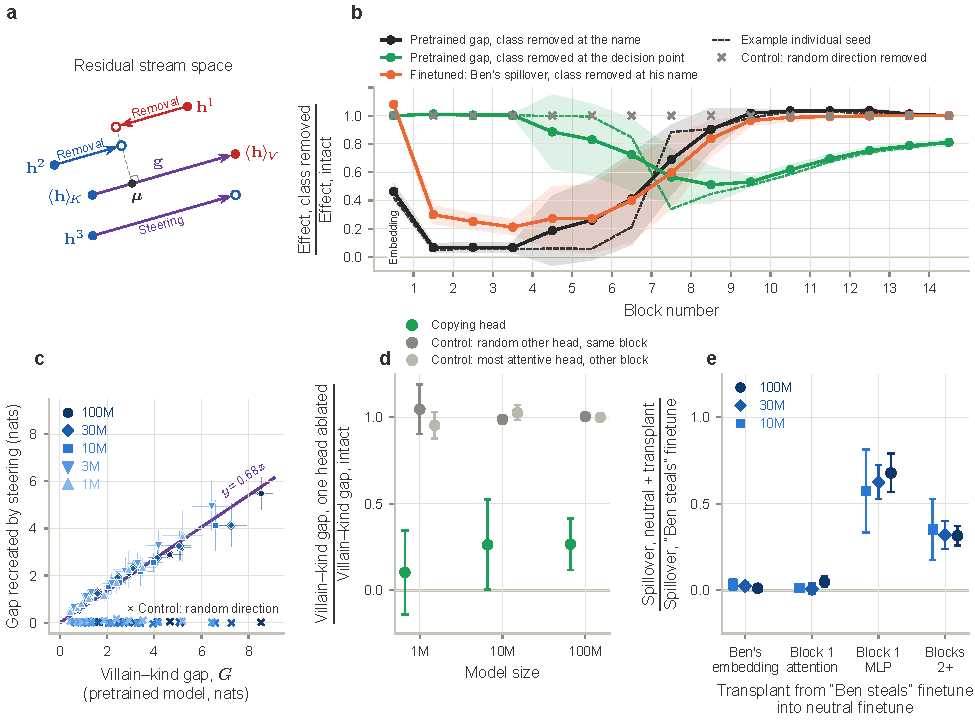
\includegraphics[width=\textwidth]{fig6_mechanism.pdf}
  \caption{
    \textbf{Interventions on activations and weights.}
    ``Villain/kind names'' at $z=0$ (\textbf{c}: $0 \le z \le 0.5$).
    Bands and error bars: 95\% CI over 8 seeds.
    Gap: villain-kind gap, as in \cref{fig:readout} (over all four acts).
    Spillover: onto ``lie,'' ``cheat,'' and ``tease'' after the ``Ben steals'' finetune (see \cref{fig:test}).
    \panel{a} Illustration of the interventions in \textbf{b} and \textbf{c}.
    $\langle\mathbf{h}\rangle_V$ and $\langle\mathbf{h}\rangle_K$: the mean residual streams of villain-name and kind-name items after a given block, at one token (\textbf{b}: the name or the decision point).
    $\mathbf{g}$: the class vector (\cref{eq:class-dir}).
    $\boldsymbol{\mu}$: the mean over all items. $\mathbf{h}^1$--$\mathbf{h}^3$: example items.
    Removal: set an item's component along $\mathbf{g}$ to match $\boldsymbol{\mu}$ (\cref{eq:remove}).
    Steering: add $\mathbf{g}$ to a kind name's embedding (\cref{eq:steer}).
    \panel{b} Locating the class (villain or kind) in the residual stream (100M models).
    The removal happens at one point in the residual stream: after the embedding, or after a transformer block, each with its own $\mathbf{g}$ (points sit between blocks).
    At the name: every token of every mention of the relevant character's name.
    At the decision point: the last token before the endings branch, and every subsequent token in both branches, except the last token.
    Dashed: seed 3 (\cref{sec:app-mechanism}).
    Control: average over 3 random directions removed at the decision point.
    \panel{c} Steering kind names toward the villain class, one point per corpus and size.
    We add $\mathbf{g}$ (here from token embeddings, over all 24 kind names) at every mention of the name being steered.
    Gap recreated by steering: score with steering minus score without.
    Control: add a vector of random direction and the same length instead.
    Line: fit through the origin (see \cref{fig:flowbyact}c).
    \panel{d} (exploratory) Attention head ablation.
    Based on each seed's largest jump in \textbf{b} (at the name, evaluated for each model size), we identify the block with the most ``copying'' to the decision point, and further find the individual attention head that copies the most.
    We plot how much of the villain-kind gap remains when mean-ablating that ``copying head.''
    For control, we compare to mean-ablating a random other head in the same block, and the head in another block that attends most from the decision point to the name.
    \panel{e} (exploratory) Transplanting parts of a finetune. We begin with a neutral finetune and overwrite part of it with weights from the corresponding ``Ben steals'' finetune.
  }
  \label{fig:mechanism}
\end{figure}
